%%
% Copyright (c) 2017 - 2021, Pascal Wagler;
% Copyright (c) 2014 - 2021, John MacFarlane
%
% All rights reserved.
%
% Redistribution and use in source and binary forms, with or without
% modification, are permitted provided that the following conditions
% are met:
%
% - Redistributions of source code must retain the above copyright
% notice, this list of conditions and the following disclaimer.
%
% - Redistributions in binary form must reproduce the above copyright
% notice, this list of conditions and the following disclaimer in the
% documentation and/or other materials provided with the distribution.
%
% - Neither the name of John MacFarlane nor the names of other
% contributors may be used to endorse or promote products derived
% from this software without specific prior written permission.
%
% THIS SOFTWARE IS PROVIDED BY THE COPYRIGHT HOLDERS AND CONTRIBUTORS
% "AS IS" AND ANY EXPRESS OR IMPLIED WARRANTIES, INCLUDING, BUT NOT
% LIMITED TO, THE IMPLIED WARRANTIES OF MERCHANTABILITY AND FITNESS
% FOR A PARTICULAR PURPOSE ARE DISCLAIMED. IN NO EVENT SHALL THE
% COPYRIGHT OWNER OR CONTRIBUTORS BE LIABLE FOR ANY DIRECT, INDIRECT,
% INCIDENTAL, SPECIAL, EXEMPLARY, OR CONSEQUENTIAL DAMAGES (INCLUDING,
% BUT NOT LIMITED TO, PROCUREMENT OF SUBSTITUTE GOODS OR SERVICES;
% LOSS OF USE, DATA, OR PROFITS; OR BUSINESS INTERRUPTION) HOWEVER
% CAUSED AND ON ANY THEORY OF LIABILITY, WHETHER IN CONTRACT, STRICT
% LIABILITY, OR TORT (INCLUDING NEGLIGENCE OR OTHERWISE) ARISING IN
% ANY WAY OUT OF THE USE OF THIS SOFTWARE, EVEN IF ADVISED OF THE
% POSSIBILITY OF SUCH DAMAGE.
%%

%%
% This is the Eisvogel pandoc LaTeX template.
%
% For usage information and examples visit the official GitHub page:
% https://github.com/Wandmalfarbe/pandoc-latex-template
%%

% Options for packages loaded elsewhere
\PassOptionsToPackage{unicode}{hyperref}
\PassOptionsToPackage{hyphens}{url}
\PassOptionsToPackage{dvipsnames,svgnames*,x11names*,table}{xcolor}
%
\documentclass[
  brazilian,
  paper=a4,
  oneside  ,captions=tableheading
]{scrbook}
\usepackage{amsmath,amssymb}

\usepackage{chngcntr}
\counterwithout{figure}{chapter}

\usepackage{lmodern}
\usepackage{setspace}
\setstretch{1.2}
\usepackage{ifxetex,ifluatex}
\ifnum 0\ifxetex 1\fi\ifluatex 1\fi=0 % if pdftex
  \usepackage[T1]{fontenc}
  \usepackage[utf8]{inputenc}
  \usepackage{textcomp} % provide euro and other symbols
\else % if luatex or xetex
  \usepackage{unicode-math}
  \defaultfontfeatures{Scale=MatchLowercase}
  \defaultfontfeatures[\rmfamily]{Ligatures=TeX,Scale=1}
\fi
% Use upquote if available, for straight quotes in verbatim environments
\IfFileExists{upquote.sty}{\usepackage{upquote}}{}
\IfFileExists{microtype.sty}{% use microtype if available
  \usepackage[]{microtype}
  \UseMicrotypeSet[protrusion]{basicmath} % disable protrusion for tt fonts
}{}
\makeatletter
\@ifundefined{KOMAClassName}{% if non-KOMA class
  \IfFileExists{parskip.sty}{%
    \usepackage{parskip}
  }{% else
    \setlength{\parindent}{0pt}
    \setlength{\parskip}{6pt plus 2pt minus 1pt}}
}{% if KOMA class
  \KOMAoptions{parskip=half}}
\makeatother
\usepackage{xcolor}
\definecolor{default-linkcolor}{HTML}{A50000}
\definecolor{default-filecolor}{HTML}{A50000}
\definecolor{default-citecolor}{HTML}{4077C0}
\definecolor{default-urlcolor}{HTML}{4077C0}
\IfFileExists{xurl.sty}{\usepackage{xurl}}{} % add URL line breaks if available
\IfFileExists{bookmark.sty}{\usepackage{bookmark}}{\usepackage{hyperref}}
\hypersetup{
  pdftitle={Lista de Exercícios 4 (Pilhas e Filas)},
  pdfauthor={Ewerton Luiz Costadelle},
  pdflang={pt-br},
  pdfkeywords={Pilha Fila Deque RPN},
  hidelinks,
  breaklinks=true,
  pdfcreator={LaTeX via pandoc with the Eisvogel template}}
\urlstyle{same} % disable monospaced font for URLs
\usepackage[margin=2.5cm,includehead=true,includefoot=true,centering,]{geometry}
\usepackage{listings}
\newcommand{\passthrough}[1]{#1}
\lstset{defaultdialect=[5.3]Lua}
\lstset{defaultdialect=[x86masm]Assembler}
\usepackage{etoolbox}
\BeforeBeginEnvironment{lstlisting}{\par\noindent\begin{minipage}{\linewidth}}
\AfterEndEnvironment{lstlisting}{\end{minipage}\par\addvspace{\topskip}}
% add backlinks to footnote references, cf. https://tex.stackexchange.com/questions/302266/make-footnote-clickable-both-ways
\usepackage{footnotebackref}
\usepackage{graphicx}
\makeatletter
\def\maxwidth{\ifdim\Gin@nat@width>\linewidth\linewidth\else\Gin@nat@width\fi}
\def\maxheight{\ifdim\Gin@nat@height>\textheight\textheight\else\Gin@nat@height\fi}
\makeatother
% Scale images if necessary, so that they will not overflow the page
% margins by default, and it is still possible to overwrite the defaults
% using explicit options in \includegraphics[width, height, ...]{}
\setkeys{Gin}{width=\maxwidth,height=\maxheight,keepaspectratio}
% Set default figure placement to htbp
\makeatletter
\def\fps@figure{htbp}
\makeatother
\setlength{\emergencystretch}{3em} % prevent overfull lines
\providecommand{\tightlist}{%
  \setlength{\itemsep}{0pt}\setlength{\parskip}{0pt}}
\setcounter{secnumdepth}{-\maxdimen} % remove section numbering

% Make use of float-package and set default placement for figures to H.
% The option H means 'PUT IT HERE' (as  opposed to the standard h option which means 'You may put it here if you like').
\usepackage{float}
\floatplacement{figure}{H}

\ifxetex
    % See issue https://github.com/reutenauer/polyglossia/issues/127
  \renewcommand*\familydefault{\sfdefault}
    % Load polyglossia as late as possible: uses bidi with RTL langages (e.g. Hebrew, Arabic)
  \usepackage{polyglossia}
  \setmainlanguage[]{}
\else
  \usepackage[main=brazilian]{babel}
% get rid of language-specific shorthands (see #6817):
\let\LanguageShortHands\languageshorthands
\def\languageshorthands#1{}
\fi
\ifluatex
  \usepackage{selnolig}  % disable illegal ligatures
\fi

\title{Lista de Exercícios 4 (Pilhas e Filas)}
\author{Ewerton Luiz Costadelle}
\date{13/06/2022}



%%
%% added
%%

%
% language specification
%
% If no language is specified, use English as the default main document language.
%



%
% for the background color of the title page
%

%
% break urls
%
\PassOptionsToPackage{hyphens}{url}

%
% When using babel or polyglossia with biblatex, loading csquotes is recommended
% to ensure that quoted texts are typeset according to the rules of your main language.
%
\usepackage{csquotes}

%
% captions
%
\definecolor{caption-color}{HTML}{777777}
\usepackage[font={stretch=1.2}, textfont={color=caption-color}, position=top, skip=4mm, labelfont=bf, singlelinecheck=false, justification=raggedright]{caption}
\setcapindent{0em}

%
% blockquote
%
\definecolor{blockquote-border}{RGB}{221,221,221}
\definecolor{blockquote-text}{RGB}{119,119,119}
\usepackage{mdframed}
\newmdenv[rightline=false,bottomline=false,topline=false,linewidth=3pt,linecolor=blockquote-border,skipabove=\parskip]{customblockquote}
\renewenvironment{quote}{\begin{customblockquote}\list{}{\rightmargin=0em\leftmargin=0em}%
\item\relax\color{blockquote-text}\ignorespaces}{\unskip\unskip\endlist\end{customblockquote}}

%
% Source Sans Pro as the de­fault font fam­ily
% Source Code Pro for monospace text
%
% 'default' option sets the default
% font family to Source Sans Pro, not \sfdefault.
%
\ifnum 0\ifxetex 1\fi\ifluatex 1\fi=0 % if pdftex
    \usepackage[default]{sourcesanspro}
  \usepackage{sourcecodepro}
  \else % if not pdftex
    \usepackage[default]{sourcesanspro}
  \usepackage{sourcecodepro}

  % XeLaTeX specific adjustments for straight quotes: https://tex.stackexchange.com/a/354887
  % This issue is already fixed (see https://github.com/silkeh/latex-sourcecodepro/pull/5) but the
  % fix is still unreleased.
  % TODO: Remove this workaround when the new version of sourcecodepro is released on CTAN.
  \ifxetex
    \makeatletter
    \defaultfontfeatures[\ttfamily]
      { Numbers   = \sourcecodepro@figurestyle,
        Scale     = \SourceCodePro@scale,
        Extension = .otf }
    \setmonofont
      [ UprightFont    = *-\sourcecodepro@regstyle,
        ItalicFont     = *-\sourcecodepro@regstyle It,
        BoldFont       = *-\sourcecodepro@boldstyle,
        BoldItalicFont = *-\sourcecodepro@boldstyle It ]
      {SourceCodePro}
    \makeatother
  \fi
  \fi

%
% heading color
%
\definecolor{heading-color}{RGB}{40,40,40}
\addtokomafont{section}{\color{heading-color}}
% When using the classes report, scrreprt, book,
% scrbook or memoir, uncomment the following line.
%\addtokomafont{chapter}{\color{heading-color}}

%
% variables for title, author and date
%
\usepackage{titling}
\title{Lista de Exercícios 4 (Pilhas e Filas)}
\author{Ewerton Luiz Costadelle}
\date{13/06/2022}

%
% tables
%

%
% remove paragraph indention
%
\setlength{\parindent}{0pt}
\setlength{\parskip}{6pt plus 2pt minus 1pt}
\setlength{\emergencystretch}{3em}  % prevent overfull lines

%
%
% Listings
%
%


%
% general listing colors
%
\definecolor{listing-background}{HTML}{F7F7F7}
\definecolor{listing-rule}{HTML}{B3B2B3}
\definecolor{listing-numbers}{HTML}{B3B2B3}
\definecolor{listing-text-color}{HTML}{000000}
\definecolor{listing-keyword}{HTML}{435489}
\definecolor{listing-keyword-2}{HTML}{1284CA} % additional keywords
\definecolor{listing-keyword-3}{HTML}{9137CB} % additional keywords
\definecolor{listing-identifier}{HTML}{435489}
\definecolor{listing-string}{HTML}{00999A}
\definecolor{listing-comment}{HTML}{8E8E8E}

\lstdefinestyle{eisvogel_listing_style}{
  language         = java,
  numbers          = left,
  xleftmargin      = 2.7em,
  framexleftmargin = 2.5em,
  backgroundcolor  = \color{listing-background},
  basicstyle       = \color{listing-text-color}\linespread{1.0}\small\ttfamily{},
  breaklines       = true,
  frame            = single,
  framesep         = 0.19em,
  rulecolor        = \color{listing-rule},
  frameround       = ffff,
  tabsize          = 4,
  numberstyle      = \color{listing-numbers},
  aboveskip        = 1.0em,
  belowskip        = 0.1em,
  abovecaptionskip = 0em,
  belowcaptionskip = 1.0em,
  keywordstyle     = {\color{listing-keyword}\bfseries},
  keywordstyle     = {[2]\color{listing-keyword-2}\bfseries},
  keywordstyle     = {[3]\color{listing-keyword-3}\bfseries\itshape},
  sensitive        = true,
  identifierstyle  = \color{listing-identifier},
  commentstyle     = \color{listing-comment},
  stringstyle      = \color{listing-string},
  showstringspaces = false,
  escapeinside     = {/*@}{@*/}, % Allow LaTeX inside these special comments
  literate         =
  {á}{{\'a}}1 {é}{{\'e}}1 {í}{{\'i}}1 {ó}{{\'o}}1 {ú}{{\'u}}1
  {Á}{{\'A}}1 {É}{{\'E}}1 {Í}{{\'I}}1 {Ó}{{\'O}}1 {Ú}{{\'U}}1
  {à}{{\`a}}1 {è}{{\'e}}1 {ì}{{\`i}}1 {ò}{{\`o}}1 {ù}{{\`u}}1
  {À}{{\`A}}1 {È}{{\'E}}1 {Ì}{{\`I}}1 {Ò}{{\`O}}1 {Ù}{{\`U}}1
  {ã}{{\~a}}1 {ë}{{\"e}}1 {ï}{{\"i}}1 {ö}{{\"o}}1 {ü}{{\"u}}1
  {Ã}{{\~A}}1 {Ë}{{\"E}}1 {Ï}{{\"I}}1 {Ö}{{\"O}}1 {Ü}{{\"U}}1
  {â}{{\^a}}1 {ê}{{\^e}}1 {î}{{\^i}}1 {ô}{{\^o}}1 {û}{{\^u}}1
  {Â}{{\^A}}1 {Ê}{{\^E}}1 {Î}{{\^I}}1 {Ô}{{\^O}}1 {Û}{{\^U}}1
  {ã}{{\~a}}1 {õ}{{\~o}}1
  {Â}{{\~A}}1 {Õ}{{\~O}}1
  {œ}{{\oe}}1 {Œ}{{\OE}}1 {æ}{{\ae}}1 {Æ}{{\AE}}1 {ß}{{\ss}}1
  {ç}{{\c c}}1 {Ç}{{\c C}}1 {ø}{{\o}}1 {å}{{\r a}}1 {Å}{{\r A}}1
  {€}{{\EUR}}1 {£}{{\pounds}}1 {«}{{\guillemotleft}}1
  {»}{{\guillemotright}}1 {ñ}{{\~n}}1 {Ñ}{{\~N}}1 {¿}{{?`}}1
  {…}{{\ldots}}1 {≥}{{>=}}1 {≤}{{<=}}1 {„}{{\glqq}}1 {“}{{\grqq}}1
  {”}{{''}}1
}
\lstset{style=eisvogel_listing_style}

%
% Java (Java SE 12, 2019-06-22)
%
\lstdefinelanguage{Java}{
  morekeywords={
    % normal keywords (without data types)
    abstract,assert,break,case,catch,class,continue,default,
    do,else,enum,exports,extends,final,finally,for,if,implements,
    import,instanceof,interface,module,native,new,package,private,
    protected,public,requires,return,static,strictfp,super,switch,
    synchronized,this,throw,throws,transient,try,volatile,while,
    % var is an identifier
    var
  },
  morekeywords={[2] % data types
    % primitive data types
    boolean,byte,char,double,float,int,long,short,
    % String
    String,
    % primitive wrapper types
    Boolean,Byte,Character,Double,Float,Integer,Long,Short
    % number types
    Number,AtomicInteger,AtomicLong,BigDecimal,BigInteger,DoubleAccumulator,DoubleAdder,LongAccumulator,LongAdder,Short,
    % other
    Object,Void,void
  },
  morekeywords={[3] % literals
    % reserved words for literal values
    null,true,false,
  },
  sensitive,
  morecomment  = [l]//,
  morecomment  = [s]{/*}{*/},
  morecomment  = [s]{/**}{*/},
  morestring   = [b]",
  morestring   = [b]',
}

\lstdefinelanguage{XML}{
  morestring      = [b]",
  moredelim       = [s][\bfseries\color{listing-keyword}]{<}{\ },
  moredelim       = [s][\bfseries\color{listing-keyword}]{</}{>},
  moredelim       = [l][\bfseries\color{listing-keyword}]{/>},
  moredelim       = [l][\bfseries\color{listing-keyword}]{>},
  morecomment     = [s]{<?}{?>},
  morecomment     = [s]{<!--}{-->},
  commentstyle    = \color{listing-comment},
  stringstyle     = \color{listing-string},
  identifierstyle = \color{listing-identifier}
}

%
% header and footer
%
\usepackage{fancyhdr}

\fancypagestyle{eisvogel-header-footer}{
  \fancyhead{}
  \fancyfoot{}
  \lhead[13/06/2022]{Lista de Exercícios 4 (Pilhas e Filas)}
  \chead[]{}
  \rhead[Lista de Exercícios 4 (Pilhas e Filas)]{13/06/2022}
  \lfoot[\thepage]{Ewerton Luiz Costadelle}
  \cfoot[]{}
  \rfoot[Ewerton Luiz Costadelle]{\thepage}
  \renewcommand{\headrulewidth}{0.4pt}
  \renewcommand{\footrulewidth}{0.4pt}
}
\pagestyle{eisvogel-header-footer}

%%
%% end added
%%

\begin{document}

%%
%% begin titlepage
%%

%%
%% end titlepage
%%

\frontmatter


{
\setcounter{tocdepth}{2}
\tableofcontents
\newpage
}
\mainmatter
\hypertarget{introduuxe7uxe3o}{%
\chapter{Introdução}\label{introduuxe7uxe3o}}

Esta lista de exercícios foi proposta pelo Prof.~Dr.~Igor Machado
Coelho, como atividade continuada do tópico Estruturas Lineares na
disciplina de Estrutura de Dados e Algoritmos, do Programa de
Pós-graduação em Ciência da Computação (PGC) da Universidade Federal
Fluminense (UFF), Campus Niterói.

O autor é servidor público no Instituto Federal de Rondônia (IFRO) -
\emph{Campus} Vilhena e atua como docente nas disciplinas da área de
Engenharia Elétrica, também é aluno, em nível de doutorado, do PGC-UFF e
participa do Projeto de Cooperação entre Instituições para Qualificação
de Profissionais de Nível Superior (PCI), firmado entre o IFRO e a UFF.

Esta lista de exercícios serviu de oportunidade para que o autor tivesse
uma introdução à orientação à objetos e estrutura de projeto utilizando
boas práticas de programação. Foi um desafio sair do pensamento de
programação estruturada, com o código em apenas um arquivo e passar a
separar as funções em arquivos e subpastas. Tanto os arquivos de
cabeçalho (.hpp) quanto as implementações (.cpp) foram separados na
subpasta ``include''.

Todos os arquivos de cabeçalho começam com diretivas
\passthrough{\lstinline!\#ifndef!} e \passthrough{\lstinline!\#define!}
que evitam referência cíclica, e finalizam com a diretiva
\passthrough{\lstinline!\#include!}, que referencia o arquivo de
implementação. A exemplo do arquivo \emph{dequeEncadeado.hpp}, abaixo:

\begin{lstlisting}[language={C++}]
#ifndef _DEQUE_ENCADEADO_HPP_
#define _DEQUE_ENCADEADO_HPP_

// [...]

#include "dequeEncadeado.cpp"
#endif
\end{lstlisting}

Seguindo as diretrizes da lista de exercícios, este documento foca mais
na lógica do que em programação. É uma discussão da proposta do
algoritmo, dos aprendizados do percurso e uma análise da complexidade
assintótica dos métodos implementados. Porém, todas as implementações
foram testadas e aprovados pelo autor, com código disponibilizado no
GitHub
{[}\textbf{https://github.com/ecostadelle/lista\_pilhas\_filas}{]}.

A seguir, cada capítulo deste documento apresenta a resposta de um
exercício.

\hypertarget{exercuxedcio-1}{%
\chapter{Exercício 1}\label{exercuxedcio-1}}

\hypertarget{a-implementauxe7uxe3o-de-um-double-ended-queue-deque-encadeado}{%
\section{a) Implementação de um Double Ended Queue (DEQUE)
encadeado}\label{a-implementauxe7uxe3o-de-um-double-ended-queue-deque-encadeado}}

A fim de responder essa questão implementei tanto o deque
\href{https://github.com/ecostadelle/lista_pilhas_filas/blob/main/include/dequeSequencial.hpp}{\textbf{sequencial}}
(as ligações para os arquivos no repositório aparecem em negrito) quanto
o
\href{https://github.com/ecostadelle/lista_pilhas_filas/blob/main/include/dequeEncadeado.hpp}{\textbf{encadeado}}.
Porém, me limitei a comentar apenas no deque
\href{https://github.com/ecostadelle/lista_pilhas_filas/blob/main/include/dequeEncadeado.hpp}{\textbf{encadeado}}
porque foi o que trouxe maior aprendizado. Antes de implementá-lo, a
alocação dinâmica era bem nebulosa para mim. Preferi utilizar o tipo
genérico, de modo que a implementação pudesse ser reaproveitada em
exercícios posteriores, a exemplo das alternativas dessa questão e do
Exercício 7, que foi em ordem cronológica o 2º exercício a ser
implementado.

Preferi, também, destinar apenas uma pasta para os arquivos Os arquivos
de cabeçalho e foram A escolha pelo tipo genérico, associado à estrutura
de diretórios

No arquivo de
\href{https://github.com/ecostadelle/lista_pilhas_filas/blob/main/include/dequeEncadeado.hpp}{\textbf{cabeçalho}},
foram definidas as estruturas necessárias para implementar o Deque
Encadeado. A primeira classe (\passthrough{\lstinline!NoDeque!}) foi o
nó, que armazena um dado do tipo genérico e dois ponteiros que apontam
para os nós anterior (\passthrough{\lstinline!*noAnterior!}) e posterior
(\passthrough{\lstinline!*noSeguinte!}).

\begin{lstlisting}[language={C++}]
template<typename TipoGenerico>
class NoDeque 
{
public:
    TipoGenerico dado;
    NoDeque<TipoGenerico> *noSeguinte; 
    NoDeque<TipoGenerico> *noAnterior;
};                 
\end{lstlisting}

O tipo genérico do dado armazenado precisa ser definido na declaração da
variável e é atribuída à classe em tempo de compilação. Inclusive tive
muitos problemas quando escolhi esse método, porque eu estava compilando
os objetos separados e vinculando-os posteriormente.

Na segunda classe (\passthrough{\lstinline!Deque!}), foram declarados em
modo privado os ponteiros que apontam apenas para dois nós, o inicial e
o final. As interfaces padrão foram declaradas em modo público, de
maneira que permitiam o acesso externo a classe.

\begin{lstlisting}[language={C++}]
template <typename TipoGenerico>
class Deque 
{
private:
    NoDeque<TipoGenerico> *inicio;
    NoDeque<TipoGenerico> *fim;
    int numeroElementos;

public:
    Deque();
    ~Deque();
    void insereInicio(TipoGenerico v);
    void insereFim(TipoGenerico v);
    int tamanho();
    TipoGenerico buscaInicio();
    TipoGenerico buscaFim();
    TipoGenerico removeInicio();
    TipoGenerico removeFim();
};
\end{lstlisting}

Os métodos tiveram seu próprio arquivo de
\href{https://github.com/ecostadelle/lista_pilhas_filas/blob/main/include/dequeEncadeado.cpp}{\textbf{implementação
(dequeEncadeado.cpp)}}. Além dos métodos solicitados através do
\passthrough{\lstinline!concept!}, foram implementados um construtor
\passthrough{\lstinline!Deque()!}, que inicia as variáveis em tempo
constante \(O(1)\), e um destrutor \passthrough{\lstinline!\~Deque()!},
que ao se invocado, percorre todos os elementos do deque, liberando a
memória e evita o ``vazamento de memória''. A complexidade do método
destrutor é linearmente depende do tamanho armazenado em
\passthrough{\lstinline!numeroElementos!} (n), ou seja, \(O(n)\)

\begin{lstlisting}[language={C++}]
#include "dequeEncadeado.hpp"

template <typename TipoGenerico>
Deque<TipoGenerico>::Deque()
{
    this->numeroElementos = 0;
    this->inicio = nullptr;
    this->fim = nullptr;
}

template <typename TipoGenerico>
Deque<TipoGenerico>::~Deque()
{
    while (this->numeroElementos > 0)
        removeInicio();
} 
\end{lstlisting}

No método \passthrough{\lstinline!insereInicio()!} um nó é criado e
alocado dinamicamente na memória, um ponteiro
(\passthrough{\lstinline!*no!}) armazena o endereço e um dado é
inserido. Caso o deque esteja vazio, os endereços de início e fim serão
os mesmo do nó recém criado. Caso contrário, o campo
\passthrough{\lstinline!noSeguinte!} do nó recém criado recebe o
endereço daquele que era o início, e o campo
\passthrough{\lstinline!noAnterior!}, daquele que era o inicio, recebe o
endereço do novo nó e o número de elementos no deque é incrementado.
Este método opera em tempo constante, ou seja, \(O(1)\).

\begin{lstlisting}[language={C++}]
template <typename TipoGenerico>
void Deque<TipoGenerico>::insereInicio(TipoGenerico v)
{
    NoDeque<TipoGenerico> *no =
        new NoDeque
        {.dado = v,
         .noSeguinte = nullptr,
         .noAnterior = nullptr};
    if (numeroElementos == 0)
    {
        inicio = fim = no;
    }
    else 
    {
        no->noSeguinte = inicio;
        inicio->noAnterior = no;
        inicio = no;
    }
    numeroElementos++;
}
\end{lstlisting}

No método \passthrough{\lstinline!insereFim()!} ocorre um procedimento
semelhante ao descrito anteriormente, porém na outra ponta. E opera,
também, em tempo constante, ou seja, \(O(1)\).

\begin{lstlisting}[language={C++}]
template <typename TipoGenerico>
void Deque<TipoGenerico>::insereFim(TipoGenerico v)
{
    NoDeque<TipoGenerico> *no =
        new NoDeque<TipoGenerico> 
        {.dado = v,
         .noSeguinte = nullptr,
         .noAnterior = nullptr};
    if (numeroElementos == 0)
    {
        inicio = fim = no;
    }
    else
    {
        no->noAnterior = fim;
        fim->noSeguinte = no;
        fim = no;
    }
    numeroElementos++;
}
\end{lstlisting}

Já os métodos \passthrough{\lstinline!tamanho()!},
\passthrough{\lstinline!buscaInicio()!} e
\passthrough{\lstinline!buscaFim()!} apenas retornam variáveis que estão
privadas, é um modo seguro de se criar uma interface. Operam em tempo
constante (\(O(1)\)).

\begin{lstlisting}[language={C++}]
template <typename TipoGenerico>
int Deque<TipoGenerico>::tamanho()
{
    return this->numeroElementos;
}

template <typename TipoGenerico>
TipoGenerico Deque<TipoGenerico>::buscaInicio()
{
    return inicio->dado;
}

template <typename TipoGenerico>
TipoGenerico Deque<TipoGenerico>::buscaFim()
{ 
    return fim->dado;
}
\end{lstlisting}

Os métodos \passthrough{\lstinline!removeInicio()!} e
\passthrough{\lstinline!removeFim()!} operam em tempo constante
(\(O(1)\)) e quando um deles é invocado, ele armazena o endereço do nó
que será removido, coleta o dado armazenado, remove o nó, decrementa o
número de elementos, define a nova ponta da fila (seja no início, seja
no fim) e retorna o valor lido.

\begin{lstlisting}[language={C++}]
template <typename TipoGenerico>
TipoGenerico Deque<TipoGenerico>::removeInicio()
{
    NoDeque<TipoGenerico> *p = inicio;
    TipoGenerico r = p->dado;
    delete p;
    numeroElementos--;
    inicio = inicio->noSeguinte;
    return r;
}

template <typename TipoGenerico>
TipoGenerico Deque<TipoGenerico>::removeFim() 
{                                             
    NoDeque<TipoGenerico> *p = fim;           
    TipoGenerico r = p->dado;
    delete p;
    numeroElementos--;
    fim = fim->noAnterior;              
    return r;
}
\end{lstlisting}

Conforme solicitado, o \passthrough{\lstinline!static\_assert!} verifica
os métodos do \passthrough{\lstinline!concept!}, algumas pequenas
alterações foram feitas: a palavra \passthrough{\lstinline!bool!} foi
removida porque os código foi implementado em C++20, uma vez que o
IntelliSense reclamou dos métodos em questão enquanto era utilizado o
C++17; a segunda alteração foi o acréscimo da palavra ``busca'' nos
métodos que realizavam essa ação, com o objetivo de melhorar a
legibilidade do código. Abaixo estão os códigos do
\passthrough{\lstinline!concept!} e do
\passthrough{\lstinline!static\_assert!}

\begin{lstlisting}[language={C++}]
template <typename Agregado, typename Tipo>
concept DequeTAD = requires(Agregado a, Tipo t)
{
    // requer operação de consulta ao elemento 'inicio'
    {a.buscaInicio()};
    // requer operação de consulta ao elemento 'fim'
    {a.buscaFim()};
    // requer operação 'insereInicio' sobre tipo 't'
    {a.insereInicio(t)};
    // requer operação 'insereFim' sobre tipo 't'
    {a.insereFim(t)};
    // requer operação 'removeInicio' e retorna tipo 't'
    {a.removeInicio()};
    // requer operação 'removeFim' e retorna tipo 't'
    {a.removeFim()};
};
// testa se Deque está correto
static_assert(DequeTAD<Deque<char>, char>);
\end{lstlisting}

\hypertarget{b-implementauxe7uxe3o-de-uma-pilha-utilizando-um-deque}{%
\section{b) Implementação de uma pilha utilizando um
DEQUE}\label{b-implementauxe7uxe3o-de-uma-pilha-utilizando-um-deque}}

No arquivo de cabeçalho
\href{https://github.com/ecostadelle/lista_pilhas_filas/blob/main/include/pilhaDeque.hpp}{\textbf{pilhaDeque.hpp}},
foram declarados, em uma classe, uma variável com o Tipo Abstrato de
Dados (TAD) Deque (definindo o tipogenérico como
\passthrough{\lstinline!char!}) e os protótipos das interfaces padrão do
TAD pilhaDeque. Preferiu-se utilizar métodos com nomes semelhantes aos
disponíveis na Biblioteca de Modelos Padrão (STL - \emph{standard
template library}) do C++.

\begin{lstlisting}[language={C++}]
#ifndef _PILHA_DEQUE_HPP_
#define _PILHA_DEQUE_HPP_

#include "dequeEncadeado.hpp"

class PilhaDeque
{
public:
    Deque<char> d; 

    PilhaDeque();
    ~PilhaDeque();
    bool empty();
    char top();
    void push(char t);
    char pop();
}; 

#include "pilhaDeque.cpp"

#endif
\end{lstlisting}

No arquivo de implementação
\href{https://github.com/ecostadelle/lista_pilhas_filas/blob/main/include/pilhaDeque.cpp}{\textbf{pilhaDeque.cpp}},
foram declarados os métodos utilizando as interfaces padrão do TAD
\passthrough{\lstinline!Deque!}, limitando-se apenas em operar em uma
das pontas. Com exceção do método destrutor, que opera em tempo
linearmente dependente do número de elementos, \(O(n)\), todos os demais
métodos operam em tempo constante \(O(1)\).

\begin{lstlisting}[language={C++}]
#include <iostream>
#include "pilhaDeque.hpp"

PilhaDeque::PilhaDeque()
{
}

PilhaDeque::~PilhaDeque()
{
    d.~Deque();
}

bool PilhaDeque::empty()
{
    return (d.tamanho() == 0);
}

char PilhaDeque::top()
{
    return d.buscaFim();
}

void PilhaDeque::push(char t)
{
    d.insereFim(t);
}

char PilhaDeque::pop()
{
    return d.removeFim();
}
\end{lstlisting}

O \passthrough{\lstinline!static\_assert!} verifica se o os métodos
solicitados pelo \passthrough{\lstinline!concept!} foram satisfeitos.

\begin{lstlisting}[language={C++}]
template <typename Agregado, typename Tipo>
concept PilhaTAD = requires(Agregado c, Tipo t)
{
    // requer operação de consulta ao elemento 'fim'
    {c.top()};
    // requer operação 'insereFim' sobre tipo 't'
    {c.push(t)};
    // requer operação 'removeFim' e retorna tipo 't'
    {c.pop()};
};
// testa se Pilha está correta
static_assert(PilhaTAD<PilhaDeque, char>);
\end{lstlisting}

\hypertarget{c-implementauxe7uxe3o-de-uma-pilha-utilizando-um-deque}{%
\section{c) Implementação de uma pilha utilizando um
DEQUE}\label{c-implementauxe7uxe3o-de-uma-pilha-utilizando-um-deque}}

No arquivo de cabeçalho
\href{https://github.com/ecostadelle/lista_pilhas_filas/blob/main/include/filaDeque.hpp}{\textbf{filaDeque.hpp}},
foram declarados, em uma classe, uma variável com o Tipo Abstrato de
Dados (TAD) Deque (definindo o tipogenérico como
\passthrough{\lstinline!char!}) e os protótipos das interfaces padrão do
TAD \passthrough{\lstinline!filaDeque!}. Assim como no exercício
anterior, preferiu-se utilizar métodos com nomes semelhantes aos
disponíveis na Biblioteca de Modelos Padrão (STL - \emph{standard
template library}) do C++.

\begin{lstlisting}[language={C++}]
#ifndef _FILA_DEQUE_HPP_
#define _FILA_DEQUE_HPP_

#include "dequeEncadeado.hpp"

class FilaDeque
{
public:
    Deque<char> d; 

    FilaDeque();
    ~FilaDeque();
    bool empty();
    char front();
    void push(char t);
    char pop();
}; 

#include "FilaDeque.cpp"

#endif
\end{lstlisting}

No arquivo de implementação
\href{https://github.com/ecostadelle/lista_pilhas_filas/blob/main/include/filaDeque.cpp}{\textbf{filaDeque.cpp}},
foram declarados os métodos utilizando as interfaces padrão do TAD
\passthrough{\lstinline!Deque!}, limitando-se apenas em inserir dados em
uma das pontas e remover na outra. Com exceção do método destrutor, que
opera em tempo linearmente dependente do número de elementos, \(O(n)\),
todos os demais métodos operam em tempo constante \(O(1)\).

\begin{lstlisting}[language={C++}]
#include <iostream>
#include "filaDeque.hpp"

FilaDeque::FilaDeque()
{
}

FilaDeque::~FilaDeque()
{
    d.~Deque();
}

bool FilaDeque::empty()
{
    return (d.tamanho() == 0);
}

char FilaDeque::front()
{
    return d.buscaInicio();
}

void FilaDeque::push(char t)
{
    d.insereFim(t);
}

char FilaDeque::pop()
{
    return d.removeInicio();
}
\end{lstlisting}

O \passthrough{\lstinline!static\_assert!} verifica se o os métodos
solicitados pelo \passthrough{\lstinline!concept!} foram satisfeitos.

\begin{lstlisting}[language={C++}]
template <typename Agregado, typename Tipo>
concept FilaTAD = requires(Agregado c, Tipo t)
{
    // requer operação de consulta ao elemento 'inicio'
    {c.front()};
    // requer operação 'insereFim' sobre tipo 't'
    {c.push(t)};
    // requer operação 'removeInicio' e retorna tipo 't'
    {c.pop()};
};
// testa se Fila está correta
static_assert(FilaTAD<FilaDeque, char>);
\end{lstlisting}

\hypertarget{exercuxedcio-2}{%
\chapter{Exercício 2}\label{exercuxedcio-2}}

\hypertarget{implementauxe7uxe3o-uma-pilha-utilizando-duas-filas.}{%
\section{Implementação uma Pilha utilizando duas
Filas.}\label{implementauxe7uxe3o-uma-pilha-utilizando-duas-filas.}}

Para resolver esse exercício pensou-se na seguinte estratégia, manter a
pilha na ordem de retirada na primeira fila e quando um novo elemento
for inserido, move-se todos os elementos para a segunda fila, insere o
elemento na primeira e retorna os elementos da segunda fila para a
primeira.

Seguindo o padrão do projeto, os arquivos de cabeçalho e implementação
foram colocados no subdiretório \passthrough{\lstinline!include!}. No
arquivo de cabeçalho
\href{https://github.com/ecostadelle/lista_pilhas_filas/blob/main/include/pilha2F.cpp}{\textbf{pilha2F.cpp}},
foi declarada uma fila genérica do STL, para armazenar o tipo
\passthrough{\lstinline!char!} e os protótipos da interface padrão do
TAD. Seguindo o que vem sendo aplicado nos exercícios anteriores,
utilizou-se métodos com nomes semelhantes aos disponíveis na STL.

\begin{lstlisting}[language={C++}]
#ifndef _PILHA_2F_HPP_
#define _PILHA_2F_HPP_

#include <queue> // Fila genérica em C++

class Pilha2F {
public:
    std::queue<char> f1; // Fila para 'char'
    std::queue<char> f2; // Fila para 'char'
    // SOMENTE espaço auxiliar CONSTANTE aqui 
    // (nenhum vetor, lista, etc) 
    // implementar métodos do TAD Pilha
    Pilha2F();
    ~Pilha2F();
    bool empty();
    char top();
    void push(char t);
    char pop();
};

#include "pilha2F.cpp"

#endif
\end{lstlisting}

No arquivo de implementação
\href{https://github.com/ecostadelle/lista_pilhas_filas/blob/main/include/pilha2F.cpp}{\textbf{pilha2F.cpp}},
foram efetivados os métodos que permitiram a operação solicitada. No
método construtor, foram inicializadas as variáveis da classe
\passthrough{\lstinline!Pilha2F!}, este método opera em tempo constante
(\(O(1)\)).

\begin{lstlisting}[language={C++}]
Pilha2F::Pilha2F()
{
    // Inicialização das filas
    f1 = std::queue<char>{};
    f2 = std::queue<char>{};
}
\end{lstlisting}

Já o método destrutor, abaixo, percorre todos os elementos da pilha e os
remove. Operando em tempo linearmente dependente do número de elementos
armazenado na pilha (n), ou seja, opera em \(O(n)\).

\begin{lstlisting}[language={C++}]
Pilha2F::~Pilha2F()
{
    while (this->empty() == false)
    {
        this->pop();
    }
}
\end{lstlisting}

O método \passthrough{\lstinline!push()!} é o mais importante desta
implementação, é nele que é executado a o algoritmo que permitiu a
operação solicitada. Quando o usuário solicita um
\passthrough{\lstinline!push!}, todos os elementos da primeira fila
(\passthrough{\lstinline!f1!}) são removidos para a segunda
(\passthrough{\lstinline!f2!}), o elemento é inserido na
\passthrough{\lstinline!f1!} e todos os elementos da
\passthrough{\lstinline!f2!} retornam para a
\passthrough{\lstinline!f1!}. Deste modo, a cada nova inserção são
necessárias operações em dobro se comparado com o número de elementos
(n), mesmo sendo \(O(2n)\), assintoticamente opera em tempo \(O(n)\).

\begin{lstlisting}[language={C++}]
void Pilha2F::push(char t)
{
    while (!f1.empty())
    {
        f2.push(f1.front());
        f1.pop();
    }

    f1.push(t);

    while (!f2.empty())
    {
        f1.push(f2.front());
        f2.pop();
    }
}
\end{lstlisting}

Manter o último elemento inserido na pilha na primeira posição da
\passthrough{\lstinline!f1!}, favorece os métodos
\passthrough{\lstinline!top()!} e \passthrough{\lstinline!pop()!} que
operarão sempre no elemento que está na frente da
\passthrough{\lstinline!f1!}. Operando sempre em tempo constante,
\(O(1)\).

\begin{lstlisting}[language={C++}]
char Pilha2F::top()
{
    return f1.front();
}

char Pilha2F::pop()
{
    char t = f1.front();
    f1.pop();
    return t;
}
\end{lstlisting}

O método \passthrough{\lstinline!empty()!} verifica se ambas filas estão
vazias. Em tese, \passthrough{\lstinline!f2!} é um espaço auxiliar e
permanece vazia em todos os métodos, com exceção do
\passthrough{\lstinline!push!}. O método
\passthrough{\lstinline!empty()!} opera em tempo constante, \(O(1)\).

\begin{lstlisting}[language={C++}]
bool Pilha2F::empty()
{
    return f1.empty() && f2.empty();
}
\end{lstlisting}

O \passthrough{\lstinline!static\_assert!} verifica se o os métodos
solicitados pelo \passthrough{\lstinline!concept!} foram satisfeitos.

\begin{lstlisting}[language={C++}]
template <typename Agregado, typename Tipo>
concept PilhaTAD2F = requires(Agregado a, Tipo t)
{
    {a.empty()};
    {a.top()};
    {a.push(t)};
    {a.pop()};
};
// testa se Pilha está correta
static_assert(PilhaTAD2F<Pilha2F, char>);
\end{lstlisting}

\hypertarget{exercuxedcio-3}{%
\chapter{Exercício 3}\label{exercuxedcio-3}}

\hypertarget{implementauxe7uxe3o-de-uma-fila-utilizando-duas-pilhas}{%
\section{Implementação de uma Fila utilizando duas
Pilhas}\label{implementauxe7uxe3o-de-uma-fila-utilizando-duas-pilhas}}

Para resolver esse exercício pensou-se na seguinte estratégia: os
elementos são inseridos (\passthrough{\lstinline!push!}) em uma pilha,
porém tanto na retirada (\passthrough{\lstinline!pop!}) quanto na
consulta da fila (\passthrough{\lstinline!front!}) faz-se necessária a
movimentação dos elementos da primeira pilha para a segunda. Ou seja, os
elementos são inseridos em tempo constante (\(O(1)\)) e removidos ou
consultados em tempo linearmente dependente do número de elementos
(\(O(n)\)).

Os arquivos de cabeçalho e implementação foram colocados no subdiretório
\passthrough{\lstinline!include!} e, mais especicamente, no arquivo de
cabeçalho
\href{https://github.com/ecostadelle/lista_pilhas_filas/blob/main/include/pilha2F.cpp}{\textbf{pilha2F.cpp}},
foram declaradas duas pilhas genéricas do STL, para armazenar o tipo
\passthrough{\lstinline!char!} e os protótipos da interface padrão do
TAD.

\begin{lstlisting}[language={C++}]
#ifndef _FILA_2P_HPP_
#define _FILA_2P_HPP_

#include <stack>

class Fila2P
{
public:
    std::stack<char> p1; // Pilha para 'char'
    std::stack<char> p2; // Pilha para 'char'
    Fila2P();
    ~Fila2P();
    void push(char c);
    char pop();
    char front();
    bool empty();
};

#include "fila2P.cpp"

#endif
\end{lstlisting}

No arquivo de implementação
\href{https://github.com/ecostadelle/lista_pilhas_filas/blob/main/include/fila2P.cpp}{\textbf{fila2P.cpp}},
foram efetivados os métodos que permitiram a operação solicitada. Assim
como nos exercícios anteriores o método destrutor percorre a fila e
elimina os valores, a fim de evitar ``vazamento de memória''.

Já as implementações mais significativas estão nos métodos
\passthrough{\lstinline!pop()!} e \passthrough{\lstinline!front()!}, que
movimentam os dados em tempo linearmente dependente do número de
elementos (n), ou seja, em \(O(n)\).

\begin{lstlisting}[language={C++}]
char Fila2P::pop()
{
    while (!p1.empty())
    {
        p2.push(p1.top());
        p1.pop();
    }
    char c = p2.top();
    p2.pop();
    while (!p2.empty())
    {
        p1.push(p2.top());
        p2.pop();
    }
    return c;
}

char Fila2P::front()
{
    while (!p1.empty())
    {
        p2.push(p1.top());
        p1.pop();
    }
    char c = p2.top();
    while (!p1.empty())
    {
        p1.push(p2.top());
    }
    return c;
}
\end{lstlisting}

O método \passthrough{\lstinline!push()!}, que opera em tempo constante
(\(O(1)\)), apenas insere elementos no topo da
\passthrough{\lstinline!p1!}.

\begin{lstlisting}[language={C++}]
void Fila2P::push(char c)
{
    p1.push(c);
}
\end{lstlisting}

O método \passthrough{\lstinline!empty()!} apenas consulta se a fila
está vazia, verificando se ambas pilhas estão vazias.

\begin{lstlisting}[language={C++}]
bool Fila2P::empty()
{
    return p1.empty() && p2.empty();
}
\end{lstlisting}

\hypertarget{exercuxedcio-4}{%
\chapter{Exercício 4}\label{exercuxedcio-4}}

\hypertarget{a-inversuxe3o-do-conteuxfado-de-uma-pilha-utilizando-uma-fila}{%
\section{a) Inversão do conteúdo de uma Pilha utilizando uma
Fila}\label{a-inversuxe3o-do-conteuxfado-de-uma-pilha-utilizando-uma-fila}}

A inversão de uma fila utilizando uma pilha é uma operação um tanto
óbvia, uma vez que operam em pontas distintas da estrutura. Bastando,
para tanto, colocar os itens da pilha na fila e retornar da fila para a
pilha.

Seguindo o padrão do projeto, os arquivos de
\href{https://github.com/ecostadelle/lista_pilhas_filas/blob/main/include/inverteF1P.hpp}{\textbf{cabeçalho}}
e de
\href{https://github.com/ecostadelle/lista_pilhas_filas/blob/main/include/inverteF1P.cpp}{\textbf{implementação}}
estão no subdiretório \passthrough{\lstinline!/include!}. No arquivo de
\href{https://github.com/ecostadelle/lista_pilhas_filas/blob/main/include/inverteF1P.hpp}{\textbf{cabeçalho}},
além das diretivas, há apenas o protótipo da função.

\begin{lstlisting}[language={C++}]
#ifndef _INVERTE_F1P_HPP_
#define _INVERTE_F1P_HPP_

#include <stack>
#include <queue>

void inverteF1P(std::queue<char>* f);

#include "inverteF1P.cpp"   

#endif
\end{lstlisting}

É no arquivo de
\href{https://github.com/ecostadelle/lista_pilhas_filas/blob/main/include/inverteF1P.cpp}{\textbf{implementação}}
que o algoritmo é realizado. Nesse arquivo o método desempilha todos os
elementos em uma fila e depois faz a operação inversa, o dobro do número
de elementos (n) determina o número de operações necessárias à inversão.
Deste modo, o método \passthrough{\lstinline!inverteP1F()!} opera em
tempo linearmente dependente do número de elemento (n), ou seja,
\(O(n)\). Não foram necessários mais espaço auxiliar, além da própria
fila permitida pelo exercício

\begin{lstlisting}[language={C++}]
void inverteF1P(std::queue<char>* f) { 
    // somente essa pilha e mais espaço auxiliar constante
    std::stack<char> p;

    while (!f->empty()) {
        p.push(f->front());
        f->pop();
    }
    while (!p.empty()) {
        f->push(p.top());
        p.pop();
    }
}
\end{lstlisting}

\hypertarget{b-inversuxe3o-do-conteuxfado-de-uma-pilha-utilizando-duas-pilhas}{%
\section{b) Inversão do conteúdo de uma Pilha utilizando duas
Pilhas}\label{b-inversuxe3o-do-conteuxfado-de-uma-pilha-utilizando-duas-pilhas}}

Pela própria estrutura da pilha, já há uma inversão ao desempilhá-la em
outra. Nesse sentido, basta executar o procedimento de desempilhar da
pilha de entrada (\passthrough{\lstinline!p!}) para a primeira pilha
auxiliar (\passthrough{\lstinline!p1!}), de \passthrough{\lstinline!p1!}
para a segunda pilha auxiliar (\passthrough{\lstinline!p2!}) e de
\passthrough{\lstinline!p2!} para \passthrough{\lstinline!p!}.

No arquivo de
\href{https://github.com/ecostadelle/lista_pilhas_filas/blob/main/include/inverteP2P.hpp}{\textbf{cabeçalho}}
foi declarado apenas o protótipo da função
(\passthrough{\lstinline!inverteP2P!}).

\begin{lstlisting}[language={C++}]
#ifndef _INVERTE_P2P_HPP_
#define _INVERTE_P2P_HPP_

#include <stack>

void inverteP2P(std::stack<char>* p);

#include "inverteP2P.cpp"

#endif
\end{lstlisting}

Já no arquivo de
\href{https://github.com/ecostadelle/lista_pilhas_filas/blob/main/include/inverteP2P.cpp}{\textbf{implementação}}
é que está o método \passthrough{\lstinline!inverteP2P()!}, onde ocorrem
três laços, um após o outro, em que todos os elementos são obtidos,
inseridos na outra pilha e removidos. O laço acontece até que a pilha de
origem esteja vazia. Deste modo, as operações são linearmente
dependendente do número de elementos (\(n\)) na pilha de entrada, ou
seja, \(O(n)\).

\begin{lstlisting}[language={C++}]
void inverteP2P(std::stack<char> *p)
{
    std::stack<char> p1; // primeira pilha auxiliar
    std::stack<char> p2; // segunda pilha auxiliar
    // mais espaço auxiliar constante

    while (!p->empty())
    {
        p1.push(p->top());
        p->pop();
    }
    while (!p1.empty())
    {
        p2.push(p1.top());
        p1.pop();
    }
    while (!p2.empty())
    {
        p->push(p2.top());
        p2.pop();
    }
}
\end{lstlisting}

\hypertarget{c-inversuxe3o-do-conteuxfado-de-uma-pilha-utilizando-uma-pilha}{%
\section{c) Inversão do conteúdo de uma Pilha utilizando uma
Pilha}\label{c-inversuxe3o-do-conteuxfado-de-uma-pilha-utilizando-uma-pilha}}

A inversão de uma pilha, utilizando outra pilha e um espaço auxiliar
constante, necessitou de muitas iterações. Pensou-se em remover o topo
da pilha inicial (\passthrough{\lstinline!p!}) e depois toda o restante
da pilha fosse colocado na pilha auxiliar
(\passthrough{\lstinline!p1!}). Após isso, o valor que estava no topo é
inserido primeiro em \passthrough{\lstinline!p!}, de modo que o conteúdo
do topo vá para a base, em seguida todos os elementos voltam para
\passthrough{\lstinline!p!}. Essa operação repetida sucessivas vezes,
como demostrado na Figura \ref{Fig:1}, é capaz de inverter a pilha com
um custo de muitas operações de movimentação de dados.

\begin{figure}
\hypertarget{Fig:1}{%
\centering
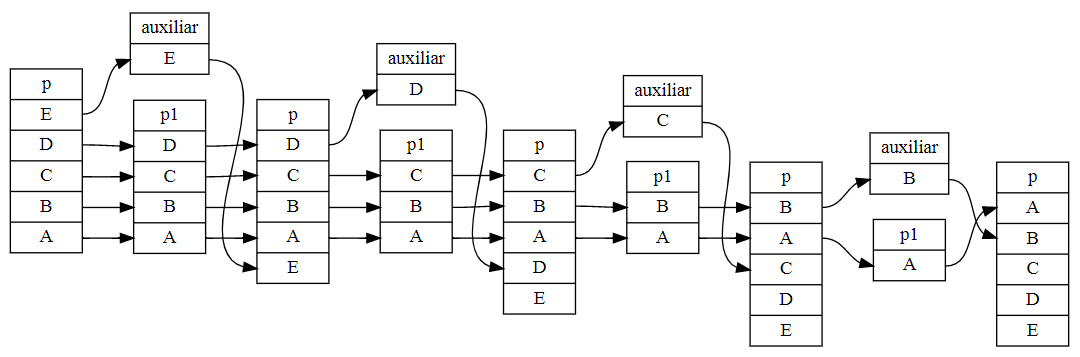
\includegraphics{inverteP1P.png}
\caption{Esquema de inversão de uma pilha utilizando outra}\label{Fig:1}
}
\end{figure}

No arquivo de
\href{https://github.com/ecostadelle/lista_pilhas_filas/blob/main/include/inverteP1P.hpp}{\textbf{cabeçalho}}
foi declarado apenas o protótipo da função.

\begin{lstlisting}[language={C++}]
#ifndef _INVERTE_P1P_HPP_
#define _INVERTE_P1P_HPP_

#include <stack>

void inverteP1P(std::stack<char>* p);

#include "inverteP1P.cpp"

#endif
\end{lstlisting}

Já no arquivo de
\href{https://github.com/ecostadelle/lista_pilhas_filas/blob/main/include/inverteP1P.cpp}{\textbf{implementação}}
é que está o método \passthrough{\lstinline!inverteP1P()!}, onde ocorre
um laço dentro de outro. O laço \passthrough{\lstinline!for!} (linha 11)
ocorre \(i\) vezes, porém \(i\) depende de \passthrough{\lstinline!--n!}
(linha 5), de modo que no laço \passthrough{\lstinline!while!} (linha 8)
ocorre \(n-1\) vezes, é possível aproximar a quantidade de iterações do
laço \passthrough{\lstinline!for!} (linha 11) para \(\frac{n-1}{2}\).
Porém, dentro do laço há duas operações de tempo constante
(\(2 \cdot \frac{n-1}{2}\)). O segundo laço
\passthrough{\lstinline!while!} (linha 15) percorre a pilha
\passthrough{\lstinline!p1!} aproximadamente \(\frac{n-2}{2}\) vezes,
devido a remoção do topo antes da entrada. Porém, dentro do laço há duas
operações de tempo constante (\(2 \cdot \frac{n-2}{2}\)). Com todas as
operações de tempo constante, a operação de inversão ocorre em
\(O(2n^2-2n+2)\), de modo que é dependente do quadrado de \(n\), os
seja, \(O(n^2)\).

\begin{lstlisting}[language={C++}]
void inverteP1P(std::stack<char>* p) { 
    std::stack<char> p1; // uma pilha auxiliar 
    // mais espaço auxiliar constante 

    int n = p->size();               // +1 
    char espacoAuxiliar;             // +1

    while(--n > 0) {                 // n-1 vezes -> (n-1)(n-1+3+n-2) 
        espacoAuxiliar = p->top();       // +1
        p->pop();                        // +1
        for (int i = 0; i < n; i++){     // (n-1)/2 vezes -> (n-1)
            p1.push(p->top());               // +1
            p->pop();                        // +1
        }
        p->push(espacoAuxiliar);         // +1
        while (!p1.empty()) {            // (n-2)/2 vezes -> (n-2)
            p->push(p1.top());               // +1
            p1.pop();                        // +1
        }
    }
}                                // O(2n^2-2n+2) = O(n^2)
\end{lstlisting}

\hypertarget{exercuxedcio-5}{%
\chapter{Exercício 5}\label{exercuxedcio-5}}

\hypertarget{a-inversuxe3o-do-conteuxfado-de-uma-fila-utilizando-uma-pilha}{%
\section{a) Inversão do conteúdo de uma Fila utilizando uma
Pilha}\label{a-inversuxe3o-do-conteuxfado-de-uma-fila-utilizando-uma-pilha}}

Pela própria estrutura da pilha, o o último elemento a ser inserido será
o primeiro elemento a ser removido. Bastando, para tanto, desenfileirar
os elementos da fila de entrada (\passthrough{\lstinline!f!}) e
empilhá-los na pilha auxiliar (\passthrough{\lstinline!p!}).

No arquivo de
\href{https://github.com/ecostadelle/lista_pilhas_filas/blob/main/include/inverteF1P.hpp}{\textbf{cabeçalho}}
foi declarado apenas o protótipo da função
(\passthrough{\lstinline!inverteF1P!}).

\begin{lstlisting}[language={C++}]
#ifndef _INVERTE_F1P_HPP_
#define _INVERTE_F1P_HPP_

#include <stack>
#include <queue>

void inverteF1P(std::queue<char>* f);

#include "inverteF1P.cpp"   

#endif
\end{lstlisting}

Já no arquivo de
\href{https://github.com/ecostadelle/lista_pilhas_filas/blob/main/include/inverteF1P.cpp}{\textbf{implementação}}
é que está o método \passthrough{\lstinline!inverteF1P()!}, onde ocorrem
dois laços, um após o outro, em que todos os elementos são obtidos,
inseridos na pilha e devolvidos para a fila.

\begin{lstlisting}[language={C++}]
void inverteF1P(std::queue<char>* f) { 
    // somente essa pilha e mais espaço auxiliar constante
    std::stack<char> p;

    while (!f->empty()) {
        p.push(f->front());
        f->pop();
    }
    while (!p.empty()) {
        f->push(p.top());
        p.pop();
    }
}
\end{lstlisting}

\hypertarget{b-inversuxe3o-do-conteuxfado-de-uma-fila-utilizando-duas-filas}{%
\section{b) Inversão do conteúdo de uma Fila utilizando duas
Filas}\label{b-inversuxe3o-do-conteuxfado-de-uma-fila-utilizando-duas-filas}}

A inversão de uma fila (\passthrough{\lstinline!f!}), utilizando outras
duas filas (\passthrough{\lstinline!f1!} e
\passthrough{\lstinline!f2!}), necessitou de muitas iterações.
Inicialmente, pensou-se em mover \(n-1\) elementos de
\passthrough{\lstinline!f!} para \passthrough{\lstinline!f2!}, em
seguida o último elemento de \passthrough{\lstinline!f!} é movido para
\passthrough{\lstinline!f1!}, feito isso, todos os elementos são
devolvidos para \passthrough{\lstinline!f!}. O processo é repetido até
que todos os elementos sejam tranferidos para
\passthrough{\lstinline!f1!}, como demostrado na \emph{Figura 2}. Esse
algoritmo é capaz de inverter a fila com um custo de muitas operações de
movimentação de dados.

\begin{figure}
\hypertarget{Fig:2}{%
\centering
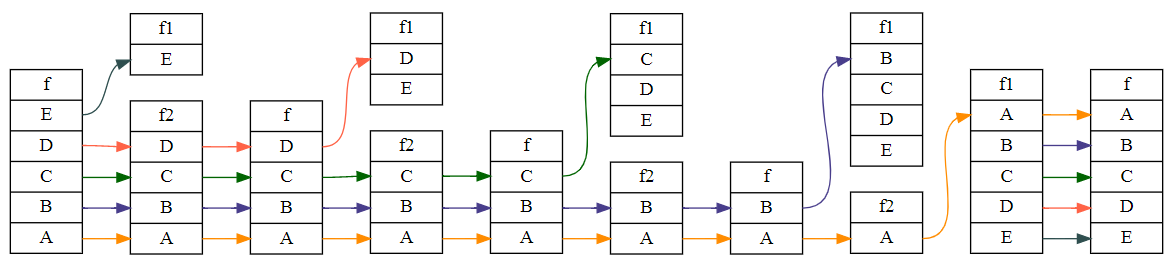
\includegraphics{inverteF2F.png}
\caption{Esquema de inversão de uma fila utilizando outras duas
filas}\label{Fig:2}
}
\end{figure}

No arquivo de
\href{https://github.com/ecostadelle/lista_pilhas_filas/blob/main/include/inverteF2F.hpp}{\textbf{cabeçalho}}
foi declarado apenas o protótipo da função
(\passthrough{\lstinline!inverteF2F!}).

\begin{lstlisting}[language={C++}]
#ifndef _INVERTE_F2F_HPP_
#define _INVERTE_F2F_HPP_

#include <queue>

void inverteF2F(std::queue<char>* f);

#include "inverteF2F.cpp"

#endif  
\end{lstlisting}

Já no arquivo de
\href{https://github.com/ecostadelle/lista_pilhas_filas/blob/main/include/inverteF2F.cpp}{\textbf{implementação}}
é que está o método \passthrough{\lstinline!inverteF2F()!}, onde ocorre
um laço dentro de outro. O laço \passthrough{\lstinline!for!} (linha 9)
ocorre \(i\) vezes, porém \(i\) depende de \passthrough{\lstinline!--n!}
(linha 8), de modo que no laço \passthrough{\lstinline!while!} (linha 8)
ocorre \(n-1\) vezes, é possível aproximar a quantidade de iterações do
laço \passthrough{\lstinline!for!} (linha 9) para \(\frac{n-1}{2}\).
Porém, dentro do laço há duas operações de tempo constante
(\(2 \cdot \frac{n-1}{2}\)). O segundo laço
\passthrough{\lstinline!while!} (linha 15) percorre a fila
\passthrough{\lstinline!f2!} aproximadamente \(\frac{n-1}{2}\) vezes.
Porém, dentro do laço há duas operações de tempo constante
(\(2 \cdot \frac{n-1}{2}\)). Com todas as operações de tempo constante,
a operação de inversão ocorre em \(O(2n^2 +1)\), de modo que é
dependente do quadrado de \(n\), os seja, \(O(n^2)\).

\begin{lstlisting}[language={C++}]
void inverteF2F(std::queue<char>* f) { 
    std::queue<char> f1; // primeira fila auxiliar 
    std::queue<char> f2; // segunda fila auxiliar 
    // mais espaço auxiliar constante 

    int n = f->size();               // +1

    while (--n > 0){                 // (n-1)->2n(n-1)=2n^2-2n
        for (int i = 0; i<n; i++){      // (n-1)/2->(n-1)
            f2.push(f->front());            // +1
            f->pop();                       // +1
        }
        f1.push(f->front());            // +1
        f->pop();                       // +1
        while (!f2.empty()) {           // (n-1)/2->(n-1)
            f->push(f2.front());            // +1
            f2.pop();                       // +1
        }
    }
    f1.push(f->front());             // +1
    f->pop();                        // +1
    while (!f1.empty()) {            // (n-1)->2(n-1)=2n-2
        f->push(f1.front());            // +1
        f1.pop();                       // +1
    }                             // 2n^2-2n+2n-2+3=2n^2+1
}
\end{lstlisting}

\hypertarget{exercuxedcio-6}{%
\chapter{Exercício 6}\label{exercuxedcio-6}}

\hypertarget{retornar-o-menor-elemento-da-pilha-em-tempo-constante}{%
\section{Retornar o menor elemento da pilha em tempo
constante}\label{retornar-o-menor-elemento-da-pilha-em-tempo-constante}}

Seguindo o padrão do projeto, no arquivo de
\href{https://github.com/ecostadelle/lista_pilhas_filas/blob/main/include/obterMinimo.hpp}{\textbf{cabeçalho}},
além das diretrizes, foram declarados uma classe
\passthrough{\lstinline!PilhaMin!}, duas pilhas, sendo uma principal
(\passthrough{\lstinline!pilhaPrincipal!}) e uma auxiliar
(\passthrough{\lstinline!pilhaAuxiliar!}). Além dos protótipos de
funções solicitados no exercício e um método
\passthrough{\lstinline!vazio()!}. Não foram necessárias outras
variáveis auxiliares.

\begin{lstlisting}[language={C++}]
#ifndef _OBTER_MINIMO_HPP_
#define _OBTER_MINIMO_HPP_

#include <stack>

class PilhaMin
{
private:
    std::stack<int> pilhaPrincipal;
    std::stack<int> pilhaAuxiliar;

public:
    // incluir variáveis necessárias
    int topo();
    int desempilha();
    void empilha(int t);
    int obterMinimo();
    // mais métodos auxiliares
    bool vazio();
};

#include "obterMinimo.cpp"

#endif
\end{lstlisting}

No arquivo de
\href{https://github.com/ecostadelle/lista_pilhas_filas/blob/main/include/obterMinimo.cpp}{\textbf{implementação}},
foram elaborados os métodos solicitados no exercício. A chave para o
funcionamento deste algoritmo está no método
\passthrough{\lstinline!empilha()!} que, cada nova inserção coloca o
valor inserido na \passthrough{\lstinline!pilhaPrincipal!} e verifica se
é menor que o mínimo registrado. Essa verificação é feita apenas
consultando o topo da \passthrough{\lstinline!pilhaAuxiliar!}. Caso
seja, o valor é empilhado também na
\passthrough{\lstinline!pilhaAuxiliar!}. Caso contrário, o valor do topo
da \passthrough{\lstinline!pilhaAuxiliar!} é repetido. Desse modo, o
topo da \passthrough{\lstinline!pilhaAuxiliar!} sempre retornará o menor
valor da \passthrough{\lstinline!pilhaPrincipal!}. O primeiro valor
inserido na pilha é empilhado em ambas as pilhas. Esse método opera em
tempo constante, \(O(1)\).

\begin{lstlisting}[language={C++}]
void PilhaMin::empilha(int t)
{
    if (pilhaPrincipal.empty())
    {
        pilhaPrincipal.push(t);
        pilhaAuxiliar.push(t);
    }
    else
    {
        pilhaPrincipal.push(t);
        if (t < pilhaAuxiliar.top())
        {
            pilhaAuxiliar.push(t);
        }
        else
        {
            pilhaAuxiliar.push(pilhaAuxiliar.top());
        }
    }
}
\end{lstlisting}

Os demais métodos de consulta e inserção de valores solicitados no
exercício também operam em tempo constante, \(O(1)\). Ao método
\passthrough{\lstinline!obterMinimo()!} coube apenas consultar o topo da
\passthrough{\lstinline!pilhaAuxiliar!}.

\begin{lstlisting}[language={C++}]
int PilhaMin::obterMinimo()
{
    return pilhaAuxiliar.top();
}
\end{lstlisting}

O método \passthrough{\lstinline!topo()!} realiza uma consulta na pilha
principal.

\begin{lstlisting}[language={C++}]
int PilhaMin::topo()
{
    return pilhaPrincipal.top();
}
\end{lstlisting}

O método \passthrough{\lstinline!desempilha()!}, retorna o valor que
está no topo, além de remover os itens das duas pilhas.

\begin{lstlisting}[language={C++}]
nt PilhaMin::desempilha()
{
    int topo = pilhaPrincipal.top();
    pilhaPrincipal.pop();
    pilhaAuxiliar.pop();
    return topo;
}
\end{lstlisting}

E o método \passthrough{\lstinline!vazio()!} apenas consulta se a
\passthrough{\lstinline!pilhaPrincipal!} está vazia.

\begin{lstlisting}[language={C++}]
bool PilhaMin::PilhaMin::vazio(){
    return (pilhaPrincipal.size()>0);
}
\end{lstlisting}

\hypertarget{exercuxedcio-7}{%
\chapter{Exercício 7}\label{exercuxedcio-7}}

\hypertarget{converter-expressuxe3o-aritmuxe9tica-em-rpn}{%
\section{Converter expressão aritmética em
RPN}\label{converter-expressuxe3o-aritmuxe9tica-em-rpn}}

Para resolver este exercício, uma pilha armazenou os operadores e um
vetor, a saída.

De modo que um laço percorre a entrada e armazena letras (variáveis)
diretamente na saída e sinais (operações) na pilha até encontrar: 1. um
parêntese fechado; ou 2. um operador de precedência inferior ao último
encontrado.

Assim que uma das duas condições é satisfeita, duas coisas podem
ocorrer, respectivamente: 1. o último operador é desempilhado, inserido
no vetor de saída, e o um parêntese aberto também é desempilhado; 2. o
operador de maior precedência é desempilhado, inserido na saída e o novo
operador é empilhado.

Ao chegar ao final do laço, todos os operadores são desempilhados e
inseridos na saída.

Com o objetivo de determinar as precedências, utilizou-se o código ASCII
do caractere subtraído de 41 em módulo 6. Esta transformação faz com que
o caractere '*' (decimal 42), torne-se 1; `+' (decimal 43), torne-se 2;
`-' (decimal 45), torne-se 4; e, por fim, o caractere `/' (decimal 47),
torne-se 0.

\backmatter
\end{document}
